\documentclass{article}

\usepackage{url} 

\usepackage{pdfpages}
\usepackage{lastpage}
\usepackage{fancyhdr}
\usepackage{ngerman}


\usepackage{floatrow}
\usepackage[tableposition=top]{caption}
\floatsetup[table]{capposition=top}

\usepackage{amsmath, amssymb}

\usepackage[utf8]{inputenc}


\usepackage[numbib]{tocbibind}

%Gummi|065|=)
\title{Oberflächenspannung}
\author{Johannes Winkler}
\date{}


\newcommand\twodigits[1]{%
   \ifnum#1<10 0#1\else #1\fi
}



\lhead{Oberflächenspannung}
\rhead{\today\\Johannes Winkler}
\cfoot{\twodigits{\thepage}~/ \pageref{LastPage}}

\begin{document}

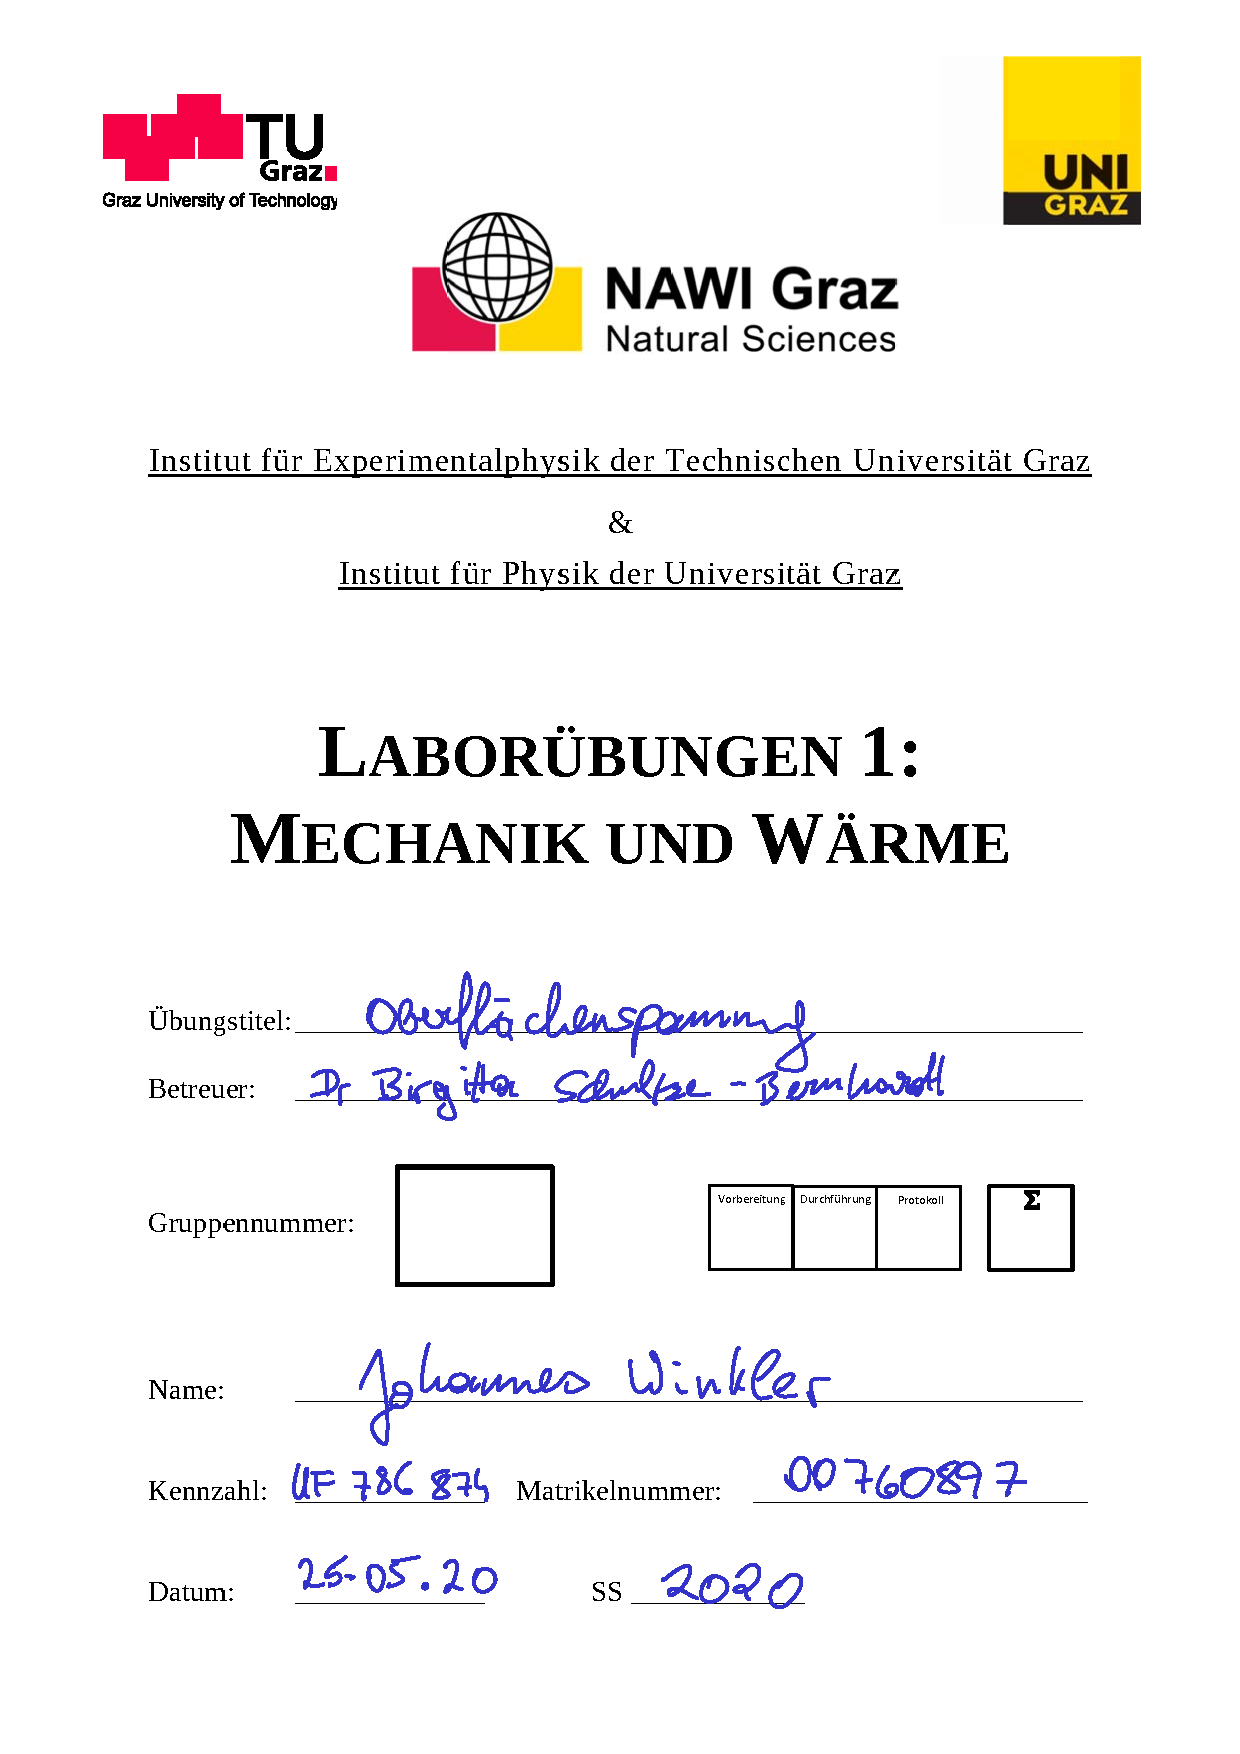
\includepdf[page=-]{deckblatt.pdf} 
 
 
\pagestyle{fancy}


\tableofcontents

\newpage


\section{Aufgabenstellung}

Bestimmung der Oberflächenspannung von Wasser und einer Seifenlösung:
\begin{itemize}
\item Mit der Bügelmethode nach Lenard bzw. mit einem Ring.
\item Aus der Steighöhe einer Kapillare.
\end{itemize}



\section{Grundlagen}

Die Oberflächenspannung $\sigma_0$ einer Flüssigkeit ist als Quotient der am Rand der Flüssigkeit
tangential zur Oberfläche angreifenden Kraft $F_R$ und der Randlänge $l_R$ definiert.

\begin{align}
\sigma_0 = F_R/l_R
\end{align}

Dies wird bei der Messung der Oberflächenspannung nach Lenard (siehe Abb. 1) realisiert. Die
Kraft $F_{VR}$ wird mit einer Federwaage gemessen, die Randlänge $l_{VR}$ ist durch die Geometrie des
Bügels gegeben. Bei der Messung mit dem Ring wird anstelle von $l_VR$ dessen Umfang eingesetzt.
Da bei dieser Methode auf zwei Seiten der Flüssigkeitshaut neue Oberfläche geschaffen wird,
ergibt sich für die Oberflächenspannung

\begin{align}
\sigma_0 = \frac{F_{VR}}{2\cdot l_{VR}}
\end{align}

Weiters kann die Oberflächenspannung auch über die Kapillaraszension (bzw. -depression) gemessen werden (siehe Abb. 2). Für eine vollständig die Innenwand der Kapillare benetzende Flüssigkeit ergibt sich für kleine Steighöhen $h$ der Flüssigkeit

\begin{align}
\sigma_0 = \frac12 \cdot r \cdot \rho \cdot g \cdot h
\end{align}

wobei $r$ der Innenradius der Kapillare, $\rho$ die Dichte der Flüssigkeit und $g = 9,81~m/s^2$ ist.


\newpage
\section{Beschreibung der Versuchsanordnung}

\begin{figure}[h]

\begin{floatrow}
\ffigbox[\FBwidth]
{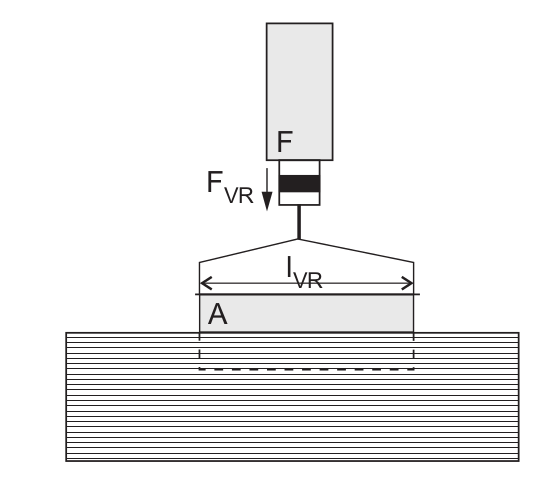
\includegraphics[height=5cm]{pic1.png}}
{\caption{Zur Messung mit dem Lenardbügel. Wird der Bügel mit Länge $l_{VR}$ aus dem Wasser gezogen, so bildet sich eine Lamelle $A$. Die dabei angreifende Kraft $F_{VR}$ wird mit einer Federwaage $F$ bestimmt.}
\label{fig:pic1}}

\ffigbox[\FBwidth]
{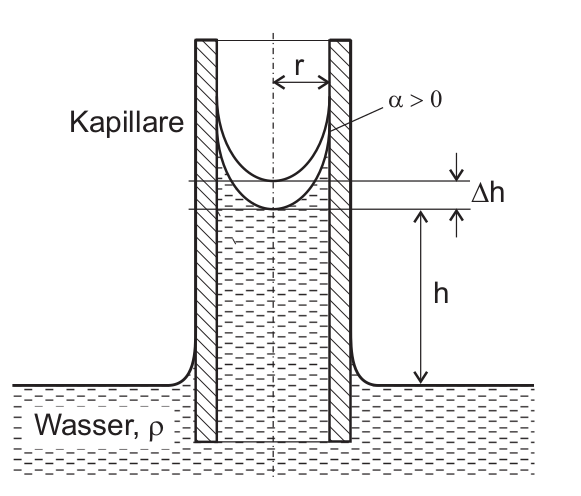
\includegraphics[height=5cm]{pic2.png}}
{\caption{Zur Messung nach der Kapillarmethode. $r$ Radius der Kapillare, $h$ Steighöhe, $\rho$ Dichte der Flüssigkeit. Für vollständig benetztende Flüssigkeiten ist der Randwinkel $\alpha=0$.}
\label{fig:pic2}}
\end{floatrow}

\end{figure}



\newpage
\section{Geräteliste}


Da aufgrund der Corona-Situation keine physikalische Anwesenheit im Labor möglich ist, kann ich auch die genauen Serien- und Gerätenummern nicht angeben.

Da auch die Gebrauchsanleitung und Datenblätter der Werkzeuge nicht vorhanden sind, werden die Messfehler dieser Geräte geschätzt.


\begin{table}[h]
\caption{Geräteliste}

\begin{tabular}{lll}
Gerät  & Gerätenummer \\
\hline
Lenardbügel  & axxxx \\
Federwaage ($\pm 1$~mN) & bxxxx \\
Metallring & cxxxx \\
Flüssigkeitsgefäß & dxxxx \\
Schiebelehre ($\pm 0.05$~mm) & exxxx \\
Schnüre zur Aufhängung & keine Nummer \\
Kapillare & gxxxx \\
Mikrometerschraube & hxxxx \\ % außendurchmesser kapillare 19:08
Kathetometer ($\pm1$~mm) & ixxxx \\ % innendurchmesser
Kapillare 1 & jxxxx \\
Kapillare 2 & kxxxx \\
Kapillare 3 & lxxxx \\
\end{tabular}
\end{table}

\newpage
\section{Versuchsdurchführung und Messergebnisse}

\subsection{Abreißmethode}

Zur besseren Reproduzierbarkeit wurde der Lenard-Bügel auf 10,035 cm gemessen. Der Durchmesser des Ringes beträgt 6 cm. Es werden jeweils 5 Messungen pro Flüssigkeit jeweils für Lenard-Bügel und Ring durchgeführt.

\begin{table}[h]
\caption{Messwerte aus der Abreißmethode: Lenard-Bügel}
\begin{tabular}{lll}
Nr. & \shortstack[l]{Kraft bei\\Wasser / mN} & \shortstack[l]{Kraft bei\\Seifenlauge / mN} \\
\hline
1 & 15,5 & 7,5 \\
2 & 15 & 8 \\
3 & 15 & 8 \\
4 & 15 & 8 \\
5 & 16 & 8
\end{tabular}
\end{table}


\begin{table}[h]
\caption{Messwerte aus der Abreißmethode: Ring}
\begin{tabular}{lll}
Nr. & \shortstack[l]{Kraft bei\\Wasser / mN} & \shortstack[l]{Kraft bei\\Seifenlauge / mN} \\
\hline
1 & 26 & 16 \\
2 & 25 & 17 \\
3 & 26 & 16 \\
4 & 26 & 16 \\
5 & 26,5 & 16
\end{tabular}
\end{table}




\subsection{Kapillarenmethode}

Bei der Kapillarenmethode kann der Innendurchmesser über den Außendurchmesser bestimmt werden. Für den Außendurchmesser der drei Kapillaren werden folgende Werte gemessen.

\begin{table}[h]
\caption{Messung der Außendurchmesser der Kapillaren und Angabe des Außenradius}

\begin{tabular}{lll}
Kapillaren & Durchmesser / mm & Außenradius / mm \\
\hline
1 & 1,77 & 0,885 \\
2 & 1,55 & 0,775 \\
3 & 1,56 & 0,780
\end{tabular}
\end{table}

Durch das Kathetometer werden die Innendurchmesser nun mit Hilfe einer dimensionslosen Skala bestimmt. Wir arbeiten über Proportionen.

\begin{table}[H]
\caption{Messung der Innendurchmesser der Kapillaren (dimensionslos)}
\label{tab:kapillaren}

\begin{tabular}{lllll|ll}
Nr. & \shortstack[l]{Beginn\\außen} & \shortstack[l]{Beginn\\innen} & \shortstack[l]{Ende\\innen} & \shortstack[l]{Ende\\außen} & \shortstack[l]{Außen-\\durchmesser} & \shortstack[l]{Innen-\\durchmesser} \\
\hline
1 & 16 & 22 & 49 & 55 & 39 & 27  \\
2 & 11 & 15 & 41 & 46 & 35 & 26 \\
3 & 18 & 23 & 48 & 53 & 35 & 25
\end{tabular}
\end{table}


Für die Bestimmung der Wasserhöhe benötigen wir einen Referenzwert, der für alle 3 Messungen gleich bleibt. Dieser wird im Video als 4,66~cm angegeben.

\begin{table}[H]
\caption{Messwerte für die Wasserhöhe in der Kapillare, Wasserhöhe relativ zum Referenzwert von 4,66~cm}
\begin{tabular}{lll}
Nr. & gemessener Wert / cm & Höhe relativ / mm\\
\hline
1 & 5,30 & 6,4 \\
2 & 5,63 & 9,7 \\
3 & 5,30 & 6,4
\end{tabular}
\end{table}


\newpage
\section{Auswertung}

\subsection{Abreißmethode: Berechnung}

Mit Hilfe der Formel 
\begin{align*}
\sigma = \frac{F}{2\cdot l}
\end{align*}
kann man nun die Oberflächenspannung $\sigma$ berechnen. Wir tun das in den folgenden Tabellen.

\begin{table}[h]
\caption{Berechnete Oberflächenspannung mit der Abreißmethode: Lenard-Bügel und $l=10,035$ cm (gerundet auf 4 Nachkommastellen zur genaueren weiteren Verwendung)}
\begin{tabular}{lll}
Nr. & \shortstack[l]{$\sigma$ bei\\Wasser / mN~m${}^{-1}$} & \shortstack[l]{$\sigma$ bei\\Seifenlauge / mN~m${}^{-1}$} \\
\hline
1 & 77,2297 & 37,3692 \\
2 & 74,7384 & 39,8605 \\
3 & 74,7384 & 39,8605 \\
4 & 74,7384 & 39,8605 \\
5 & 79,7210 & 39,8605 \\
\hline
$\overline{\sigma}$ & 76,2332 & 39,3622
\end{tabular}
\end{table}


\begin{table}[h]
\caption{Berechnete Oberflächenspannung mit der Abreißmethode: Ring und $l = 6\cdot \pi \approx 0,1885$ cm (gerundet auf 4 Nachkommastellen zur genaueren weiteren Verwendung)}
\begin{tabular}{lll}
Nr. & \shortstack[l]{$\sigma$ bei\\Wasser / mN~m${}^{-1}$} & \shortstack[l]{$\sigma$ bei\\Seifenlauge / mN~m${}^{-1}$} \\
\hline
1 & 68,9655 & 42,4403 \\
2 & 66,3130 & 45,0928 \\
3 & 68,9655 & 42,4403 \\
4 & 68,9655 & 42,4403 \\
5 & 70,2918 & 42,4403 \\
\hline
$\overline{\sigma}$ & 68,7003 & 42,9708
\end{tabular}
\end{table}


\subsection{Abreißmethode: Größtunsicherheitsmethode}

Wir setzen $\Delta l = 0,00005$ m aufgrund der Beschaffenheit der Schiebelehre. Beim Ring müssen wir diesen Wert noch mit $\pi$ multiplizieren, da wir den Umfang nicht direkt messen, sondern berechnen. Wir haben keine Angaben über die Genauigkeit der Federwaage, daher nehmen wir die Spannweite der Daten an. 

\begin{align*}
\Delta\sigma &= \left| \frac{\partial \sigma}{\partial F}\right| \cdot \Delta F + \left| \frac{\partial \sigma}{\partial l}\right| \cdot \Delta l \\
&= \frac{\Delta F}{2\cdot l} + \frac{F}{2\cdot  l^2}\cdot \Delta l
\end{align*}

Wir erhalten nun folgene Unsicherheiten:
\begin{itemize}
\item Lenard-Bügel im Wasser $\overline{F} = 15,3$ mN. Die maximale Spannweite unter den Messwerten beträgt $\Delta F = 1$ mN.
\begin{align*}
\Delta\sigma &= \frac{1}{2\cdot 0,10035} + \frac{15,3}{2\cdot  0,10035^2}\cdot 0,00005 =5,0205~\text{mN~m}^{-1}
\end{align*}
\item Lenard-Bügel in Seifenlauge $\overline{F} = 7,9$ mN. Die maximale Spannweite unter den Messwerten beträgt $\Delta F = 0,5$~mN.
\begin{align*}
\Delta\sigma &= \frac{0,5}{2\cdot 0,10035} + \frac{7,9}{2\cdot  0,10035^2}\cdot 0,00005 =2,5109~\text{mN~m}^{-1}
\end{align*}

\item Ring im Wasser $\overline{F} = 25,9$ mN. Die maximale Spannweite unter den Messwerten beträgt $\Delta F = 1,5$ mN.
\begin{align*}
\Delta\sigma &= \frac{1,5}{2\cdot 0,1885} + \frac{25,9}{2\cdot  0,1885^2}\cdot 0,00005\cdot 3,1416 = 4,036~\text{mN~m}^{-1}
\end{align*}

\item Ring in Seifenlauge $\overline{F} = 16,2$ mN. Die maximale Spanweite unter den Messwerten beträgt $\Delta F = 1$ mN.
\begin{align*}
\Delta\sigma &= \frac{1}{2\cdot 0,1885} + \frac{16,2}{2\cdot  0,1885^2}\cdot 0,00005\cdot 3,1416 = 2,6883~\text{mN~m}^{-1}
\end{align*}
\end{itemize}




\subsection{Kapillarenmethode: Berechnung der Innenradien}

Bei einem Außenradius von $R$ und einem Innenradius von $r$ gilt allgemein
\begin{align*}
\frac{R}{r} = \frac{\text{Außendurchmesser}}{\text{Innendurchmesser}}
\end{align*}
wobei wir den Außen- bzw Innendurchmesser aus Tabelle \ref{tab:kapillaren} beziehen.


\begin{table}[h]
\caption{Auswertung der Radien der Kapillaren}
\begin{tabular}{llll|l}
Nr. & \shortstack[l]{Außen-\\radius / mm} & \shortstack[l]{Außen-\\durchmesser} & \shortstack[l]{Innen-\\durchmesser} & \shortstack[l]{Innen-\\radius / mm} \\
\hline
1 & 0,885 & 39 & 27 & 0,6127 \\
2 & 0,775 & 35 & 26 & 0,5757 \\
3 & 0,780  & 35 & 25 & 0,5571
\end{tabular}
\end{table}


\subsection{Kapillarenmethode: Berechnung der Oberflächenspannung}


Die Formel für die Oberflächenspannung beträgt
\begin{align*}
\sigma = \frac12 \cdot r\cdot \rho \cdot g \cdot h
\end{align*}

Entsprechend ergeben sich folgende Werte

\begin{table}[H]
\caption{Berechnung der Oberflächenspannung bei der Kapillarenmethode}

\begin{tabular}{ll}
Nr. & \shortstack[l]{Oberflächen-\\spannung / N m${}^{-1}$} \\
\hline
1 & 19,1993 \\
2 & 27,3418 \\
3 & 17,4571 \\
\hline
$\overline{\sigma}$ & 21,3327
\end{tabular}
\end{table}
Da sich die Ergebnisse von Kapillare 2 und 3 um den Faktor 1,56 unterscheiden, lässt sich darauf schließen, dass diese Methode sehr gut für Messfehler ist.

\subsection{Kapillarenmethode: Größtunsicherheitsmethode}

Wir haben die Größen $r$ und $h$ gemessen, während $g = 9,81~$m/s${}^2$ und $\rho=998,2067~$kg/m${}^3$ als konstant angenommen werden (nach \cite{wikipedia}). Die Messunsichehreit der Mikrometerschraube können wir theoretisch mit $\Delta d = 1~\mu $m annehmen. Entsprechend wäre die theoretische Messunsicherheit beim Radius halbiert. Da wir allerdings beim Ablesen der Skala und beim berechnen der Schlussrechnung weitere Ungenauigkeiten haben, schätzen wir die Ungenauigkeit des Radius auf $\Delta r = 0,5 \cdot 10^{-4}~$m.

Beim Kathetometer nehmen wir einen größeren Messunsicherheit an, um auch ggf Ablesefehler zu kompensieren. Dieser sei in unserem Fall $\Delta h = 10^{-3}~$m.

\begin{align*}
\Delta \sigma &= \left|\frac{\partial \sigma}{\partial r}\right| \cdot \Delta r + \left|\frac{\partial \sigma}{\partial h}\right| \cdot \Delta h \\ 
&= \frac12 \cdot \Delta r \cdot \rho \cdot g \cdot h + \frac12 \cdot r \cdot \rho \cdot g \cdot \Delta h \\
&= \frac12 \cdot \rho \cdot g \cdot \left( \Delta r \cdot h + \Delta h \cdot r\right) \\
&= \frac12 \cdot 998,2067 \cdot 9,81 \cdot \left( 0,5\cdot 10^{-4} \cdot h + 10^{-3} \cdot r\right)
\end{align*}

Für $r$ und $h$ geben wir die maximalen Werte an. Für die Abweichung gilt dann
\begin{align*}
\Delta \sigma &= \frac12 \cdot 998,2067 \cdot 9,81 \cdot \left(0,5\cdot 10^{-4} \cdot 0,0097 + 10^{-3} \cdot 0,0006127\right)\\
&\approx 5,3735~< \text{mN}~\text{m}^{-1} 
\end{align*}


\newpage
\section{Zusammenfassung und Diskussion}

Die Oberflächenspannung wird in der Literatur \cite{demtr1} und \cite{giancoli} besprochen. Eine genaue Tabelle ist Wikipedia zu entnehmen, wo für Wasser bei 20~${}^\circ C$ eine Oberflächenspannung von $\sigma = 72,75~$mN$~$m${}^{-1}$ angegeben ist (siehe \cite{wikipedia2}). Dadurch zeigt sich, dass die Kapillaren nicht so genaue Ergebnisse liefern, wie man durch die Abreissmethode erreichen kann.

Zusammenfassend lassen sich folgende Messergebnisse feststellen

~

Lenard-Bügel mit Wasser bzw. Seifenlauge
\begin{align*}
\sigma_{\text{Wasser}} &= (76,2332 \pm 5,03)~\text{mN}~\text{m}^{-1}\\
\sigma_{\text{Seife}} &= (39,3622 \pm 2,52)~\text{mN}~\text{m}^{-1}\\
\end{align*}




Ring mit Wasser bzw. Seifenlauge
\begin{align*}
\sigma_{\text{Wasser}} &= (68,7003  \pm 4,04)~\text{mN}~\text{m}^{-1}\\
\sigma_{\text{Seife}} &= (42,9708 \pm 2,69)~\text{mN}~\text{m}^{-1}\\
\end{align*}



Für den Versuch mit den Kapillaren ergibt sich
\begin{align*}
\sigma_{\text{Wasser}} &= (21,3327 \pm 5,38)~\text{mN}~\text{m}^{-1}
\end{align*}


Wie zu erwarten gibt es für die Methode mit den Kapillaren die größte Abweichung. Es zeigt sich, dass die Abreissmethode genauer ist, und hier sollte gemäß meiner Vermutung die Methode mit dem Bügel genauer sein. Die hohe Abweichung bei der Kombination aus Wasser und Lenard-Bügel ließe sich durch einen Ausreiser erklären. Zusätzlich konnte ich die Genauigkeiten der Messinstrumente nur schätzen, da deren Genauigkeit aus dem Video nicht hervorging. 

Ein weiteres aufgetretenes Problem ist, dass mein 10 Jahre alter Laptop einen schlechten Bildschirm mit niedriger Auflösung hat und ich die genauen Messwerte am Bildschirm nur schwer erkennen konnte.

\begin{thebibliography}{9}
\bibitem{demtr1} W. Demtröder, \emph{Experimentalphysik 1: Mechanik und Wärme}, Springer-Spektrum, 8. Auflage, 2018.

\bibitem{giancoli} D. Giancoli, \emph{Physik}, Pearson, 4. Auflage, 2019.

\bibitem{wikipedia} \url{https://de.wikipedia.org/wiki/Eigenschaften_des_Wassers} (Stand: \today) 


\bibitem{wikipedia2} \url{https://de.wikipedia.org/wiki/Oberflächenspannung} (Stand: \today) 
\end{thebibliography}

\end{document}
